%%
%% This is file `sample-sigplan.tex',
%% generated with the docstrip utility.
%%
%% The original source files were:
%%
%% samples.dtx  (with options: `sigplan')
%% 
%% IMPORTANT NOTICE:
%% 
%% For the copyright see the source file.
%% 
%% Any modified versions of this file must be renamed
%% with new filenames distinct from sample-sigplan.tex.
%% 
%% For distribution of the original source see the terms
%% for copying and modification in the file samples.dtx.
%% 
%% This generated file may be distributed as long as the
%% original source files, as listed above, are part of the
%% same distribution. (The sources need not necessarily be
%% in the same archive or directory.)
%%
%% The first command in your LaTeX source must be the \documentclass command.
\documentclass[sigplan,screen]{acmart}
\settopmatter{printacmref=false}
\renewcommand\footnotetextcopyrightpermission[1]{}
% NOTE that a single column version is required for submission and peer review. This can be done by changing the \doucmentclass[...]{acmart} in this template to 
% \documentclass[manuscript,screen]{acmart}

%%
%% \BibTeX command to typeset BibTeX logo in the docs


%% Rights management information.  This information is sent to you
%% when you complete the rights form.  These commands have SAMPLE
%% values in them; it is your responsibility as an author to replace
%% the commands and values with those provided to you when you
%% complete the rights form.


%% These commands are for a PROCEEDINGS abstract or paper.



%%
%% Submission ID.
%% Use this when submitting an article to a sponsored event. You'll
%% receive a unique submission ID from the organizers
%% of the event, and this ID should be used as the parameter to this command.
%%\acmSubmissionID{123-A56-BU3}

%%
%% The majority of ACM publications use numbered citations and
%% references.  The command \citestyle{authoryear} switches to the
%% "author year" style.
%%
%% If you are preparing content for an event
%% sponsored by ACM SIGGRAPH, you must use the "author year" style of
%% citations and references.
%% Uncommenting
%% the next command will enable that style.
%%\citestyle{acmauthoryear}

%%
%% end of the preamble, start of the body of the document source.
\begin{document}

%%
%% The "title" command has an optional parameter,
%% allowing the author to define a "short title" to be used in page headers.
\title{Sentiment Analysis - An Intelligent User Interface}

%%
%% The "author" command and its associated commands are used to define
%% the authors and their affiliations.
%% Of note is the shared affiliation of the first two authors, and the
%% "authornote" and "authornotemark" commands
%% used to denote shared contribution to the research.


\author{Gaurav Kapadiya}
\email{gaurav.kapadiya@stud.fra-uas.de}
\affiliation{%
  \institution{Frankfurt university of  applied sciences}
  \streetaddress{1 Th{\o}rv{\"a}ld Circle}
  \city{Frankfurt}
  \country{Hessen}}


\author{ Kshitij Yelpale}
\email{kshitij.yelpale@stud.fra-uas.de}
\affiliation{%
  \institution{Frankfurt university of  applied sciences}
  \city{Frankfurt}
  \country{Hessen}
}



\author{Pranay Raman }
\email{pranay.raman@stud.fra-uas.de}
\affiliation{\institution{Frankfurt university of   applied sciences}
 \city{Frankfurt}
  \country{Hessen}
  }



\author{Safir Mohammad Shaikh}
\email{safir.shaikh@stud.fra-uas.de}
\affiliation{\institution{ Frankfurt university of  applied sciences}
 \city{Frankfurt}
  \country{Hessen}
}

\author{Shubham Girdhar}
\email{shubham.girdhar@stud.fra-uas.de}
\affiliation{%
  \institution{Frankfurt university of  applied sciences}
  \city{Frankfurt}
  \state{Hessen}
}


\begin{abstract}
In this era of technology, sentiment classification is an interesting and major topic in the field of Natural Language Processing (NLP). Data-driven methods, including machine learning and deep learning techniques provide effective solutions for the sentiment classification problem. While there has been a lot of research on various machine learning models to improve the accuracy of the task, there has been no comparison, based on statistical measures, between the best of models, particularly for longer texts. Therefore, we reconstruct the classification task for long reviews as a comparison problem and compare two models known to work well, Long Short-Term Memory (LSTM) and Naive Bayes. The study is constructed as a intelligent user interface which displays movie reviews and uses user feedback to measure the performance of both models. Analyzing the data collected, we show that LSTMs give significantly better results as compared to Naïve Bayes. These results suggest that LSTM based models are better than Naïve Bayes for long text sentiment classification.
\end{abstract}


%%
%% Keywords. The author(s) should pick words that accurately describe
%% the work being presented. Separate the keywords with commas.
\keywords{  sentiment analysis, LSTM, Naive Bayes }


 
\maketitle

\section{Introduction}
                       In the new time period, Internet innovation has incredibly impacted human lives . There are audit remarks accessible for each service or item that exists in our every day life on the Internet. The opinions extracted from the audit remarks become progressively significant for vendors to break down and extend their business . On one hand, client audits mirror the quality and issues of items, which is significant for the vendors. On the other hand, the number of review reports can be enormous and from alternate points of view, it is hard to evaluate all the survey reports physically. As a traditional research subject in the field of natural language processing (NLP), sentiments analysis targets mining client's mentalities and observations (for example, positive, negative or neutral) from text descriptions created by client awareness. In this manner, sentiment analysis is additionally called opinion mining and perspective investigation, which has been generally concentrated in web based business sites, social networks and different fields [1].
                       
                       Sentiment analysis is an examination field to analyse people’s subjective sentiments. for example, feelings, assessments, conclusions and mentalities towards items, administrations, associations, occasions, subjects and their characteristics. Text sentiment analysis task is one of the most significant assignments in the field of natural language processing. It is discovered that the neural system model which depends on Long Short-Term Memory (LSTM) can effectively extract the context relations of sentences [2]. The classification exactness of the model can be improved by presenting Attention Mechanism which filter irrelevant data. 
                       
                       
We know from the previous work that opinion analysis is a part of the data mining process that can observe public educe about various topics and products[3]. It is likewise the stem of natural language processing, text analysis, computational linguistics, bio-measurements, AI strategies. Example: Twitter is the second biggest social networking platform after Facebook which generates 347,222 tweets every minute and 21 million tweets per hour [1]. So it creates an opportunity for data mining and sentiment analysis based on users tweet. Twitter is limited to 140 characters of text that’s why users can explain their brief ideas via a short message [4]. Tweets have positive, negative, neutral (neither positive nor negative) sentiments, which can be mined to draw some meaningful business conclusion.


The solution could be to outsource the sentiment analysis to machine learning methods. The sentiments could be classified into different classes and meanings could be derived. For long text data, LSTM a special type of recurrent neural network , has achieved great success in solving many problems. LSTM network introduces a self- cycling mechanism that makes it easier to learn long-term dependent information than a simple cycling structure[2]. 


A basic task in sentiment analysis is classifying the polarity of a given text whether the expressed opinion is positive, negative or neutral. More Advanced, “beyond polarity” sentiment classification looks, for instance, at emotional states such as “angry”, “sad” and “happy”. We always like when YouTube recommends our favourite videos automatically, or when the restaurant works on our reviews and facilitates with better results next time we visit. Until and unless your customers are happy and interestingly interacting, your business is up and running. The User Comments/Reviews contain crucial information which cannot be ignored. By analysing the user sentiments, we can improve the user experience by providing better results.


Firstly we want to build an application with different machine learning models for text classification of English language user sentiments. The models accurately extracts people’s opinions from a large number of unstructured review texts and classifies them into sentiment classes, positive or negative! (Model Training).We would like to use top Classification techniques such as recurrent neural networks and traditional methods and compare the results. LSTM is better in analysing emotion of long sentences and can produce better accuracy rate and recall rate. It can get complete sequence and information effectively. So, we would like to use LSTM and Bayes for our classification problem. This application design can further be extended to be used in multiple specific applications like Recommender Systems, Hotel/Restaurant Review Analysis. 




\section{Related work }
In this era of big data, we have data or information about offices and administrations given by the supplier. We attempt to gather different sorts of reviews, feedback in type of text, for example, remarks, emotions, expression or any article and afterward need to give a summarization genuine result in short substance.


\subsection{Multi task classification}
As a significant subject in the NLP field, sentiment classification consistently is an interesting and vital exploration point. With the expanding popularity of deep learning, an expanding number of NLP assignments depend on word embeddings. In 2013, Google opened word2vec, a tool for computing word vectors. It can map words to low-dimensional vector space, reduce the expense of figuring, and make words to be identified with one another as opposed to free. It is a decent distributed representation strategy [1], which defeats the defect of one-hot encoding discrete representation.


The motivation behind the sentiment analysis task is to acquire the sentiment polarity contained in the sentence, while the sentence data contained in the word is not finished, so the sentence encoder is expected to remove the highlights of the sentence in order to create the vector presentation of the sentence. Convolutional Neural Networks (CNN) was initially applied in the field of picture, yet it has additionally been broadly applied in the field of NLP as of late and has accomplished great outcomes [1].

The system structure of deficient association and weight sharing reduces the multifaceted nature of the model. The presence of a convolutional layer makes CNN great at catching spatial nearby relationship and the pooling layer in the system can extraordinarily decrease the calculation [1]. The presence of word2vec makes it workable for CNN to apply to the content, empowering CNN to acquire nearby data in the content and direct feeling arrangement. Comparative works use CNN extensions to characterize sentiment and has finished multi-class classification tasks with great outcomes. 


In theory, the RNN language model could cover the time request structure of the entire content, and manage long-term dependence issues. In the practice, however, RNN could not get familiar with the information effectively [5]. At the point where the interval between the overall data of writings and the current location to be anticipated turns out to be huge, few issues will come out. As there are too many unfold layers in the Back Propagation Through time (BPTT) optimization algorithm which prompts history data misfortune and angle weakening while at the same time preparing [5]. To defeat this trouble, few researchers set forward a procedure named Long Short Term Memory (LSTM), which prompts better exploratory outcomes in some application situations [5].


\subsection{Word Embeddings}
Great word installing is the basis of the characteristic language handling task. As far as improving the quality of word vectors, Mikolov et al. [6] and Pennington [7] first found that the word vectors learned through a RNN have intresting direct substructures conducted an exhaustive preparing of the worldwide word-word co-occurrence of measurable information from the corpus and the subsequent worldwide vector (GloVe) shows interesting straight base with regards to word vector space like [8]. Maas et al. [9] took in the word embeddings with conclusion dependent on the old style neuro- probabilistic language model [9]. Tang et al. [10] proposed three models, considering the passionate propensity of text, and learning the word embeddings with feeling. In their analyses, they likewise utilize the GloVe to get introductory word embeddings. they first use assumption vocabulary as the additional data to pretrain a word sentiment classifier and afterward get the sentiment embedding of each word including the words not in sentiment dictionary. Concatenating the word inserting and its sentiment embedding can improve the nature of word embeddings. 

\subsection{Semantic Compositions}
However, the word embeddings can just speak to a singular word. For an expression or an article, it is important to consider how to combine singular word embeddings into a representation of an expression or an article. This requires consideration of the issue of semantic creation. Socher et al. [11,15] utilize Recursive Auto-encoders (RAE) to get a sequence representation of the whole content through a constant recursive combination [11,15]. In any case, so as to get a successive representation, firstly, we have to parse the sentence structure, or utilize a greedy strategy, combining and refactoring the words with the least mistake each recursive. Kim [14] propose a CNN design for text categorization, which has numerous channels of various sizes and two distinct channels. Cho et al. [12] use RNN to process text into an arrangement of words, considering the request for the words in the content.


Since the word embeddings can just represent a single word, sentence and record representations need to think about the semantic mix issue. Semantic combination models incorporate RAE [11], CNN [14] and RNN [12]. Among every one of these models, RNN with LSTM unit [13] is generally utilized in text grouping preparing, on account of the capacity in displaying long successive data sources or outputs. It is unequivocally intended for maintaining a strategic distance from the gradient vanishing issue.

\subsection{Summary}
Past work in LSTM give data with the information that NLP field grew the popularity of deep learning, and NLP assignments relies upon word embedding[1].we can likewise apply CNN to the field of picture, yet it has furthermore been comprehensively applied in the field of NLP starting late and has achieved incredible outcomes. As hypothetically RNN language model handle the time the executives of the whole content. Concatenating the word inserting and it's sentiment implanting can improve the idea of word embeddings[16]. word embeddings works just for single word while semantic arrangements work for expression or for an article, and furthermore work to make sentences from the word it is very helpful in representation of the semantic issue[12].


In the following, we need to make simple content classification with the assistance of various sort of algorithms and mechanisms. We likewise need to work away at the content of words, sentences ,feelings and can take a try at emojis, understanding as to what they describe on the feedback or on survey. If we compare past work and our work then we can easily say that although there has been some very useful work done on improving the efficiency of various machine learning models for natural language processing, our work stands out in the way that it compares two methods for a specific use case i.e. long texts.


\section{Method}
Commonly, the significant remarks/surveys of users/ customers are overlooked which contain critical data. We cannot process each audit/remark physically on the grounds that it takes a lot of efforts and sometimes it waste our valuable time. We need to face various challenges, for example, Irony, Sarcasm, Emojis, Comparisons and so on while text summarization.


\subsection{Study Design}
Our hypothesis (H1) is that LSTM outperforms Bayes model for sentiment classification, particularly for longer reviews. Null hypothesis (H0) is that there is not significant difference between LSTM and Bayes predictions. We used an interactive web application to test this hypothesis. A single factor within-subject experiment was carried out with discrete independent variable MODEL TYPE and continuous dependent variable ACCURACY. Many models could be used for sentiment classification. For the purpose of this study, we chose two of the models already known to perform well. So, the independent variable has two levels namely LSTM and Bayes.

\subsection{Implementation}
Streamlit library of python was used to design the user interface. Each participant saw 5 text areas with random long movie reviews, selected randomly from a SQLite database already containing a set of 4500 reviews. Below each review there was a slider which the user could adjust to rate the sentiment of the review (0 being negative and 1 being positive). After rating all the reviews, the participant was supposed to click the submit button. Upon clicking the button, participant's data was updated in a database which kept track of the ratings by the user, the actual rating of the review, deviation of LSTM and Bayes values from the actual value. Flask SQLAlchemy was used to create the backend database connections and APIs. The collected data was then used for statistical testing using python.

Github: \url{https://github.com/kshitijyelpale/HMI-Sentiment-Analysis-An-Intelligent-User-Interface}

% The participants saw multiple text areas where they could enter their reviews. There was a button to submit the reviews. The submitted reviews were fed to both the LSTM and BAYES models and a sentiment classification was obtained. All this data was stored in a SQLite database. A sentiment to be displayed was returned to the user-interface for each user-review. Finally, the participant was displayed a slider wherein he/she could give a value for his/her sentiments. This actual sentiment value was also stored in the database. Predicted values and actual value from participants were used to calculate the performance metric. This metric, in turn, was used for statistical testing.

\subsection{Model}
Two machine learning models were created for same operation (Sentiment Analysis). 1. LSTM Model 2. Bayes Model.For implementing these models, we used imdb movie review dataset, python libraries like keras, sklearn, tensorflow, nltk, models. The data was pre-processed (stop words, special characters. removed) and transformed to one-hot representation. Models were created, trained and evaluated for both LSTM and Bayes. The LSTM model consisted of 3: layers Embedding, LSTM and Dense. The models predicted the review and gave real valued outputs which indicate classified value of sentiments.


\begin{figure}[h]
    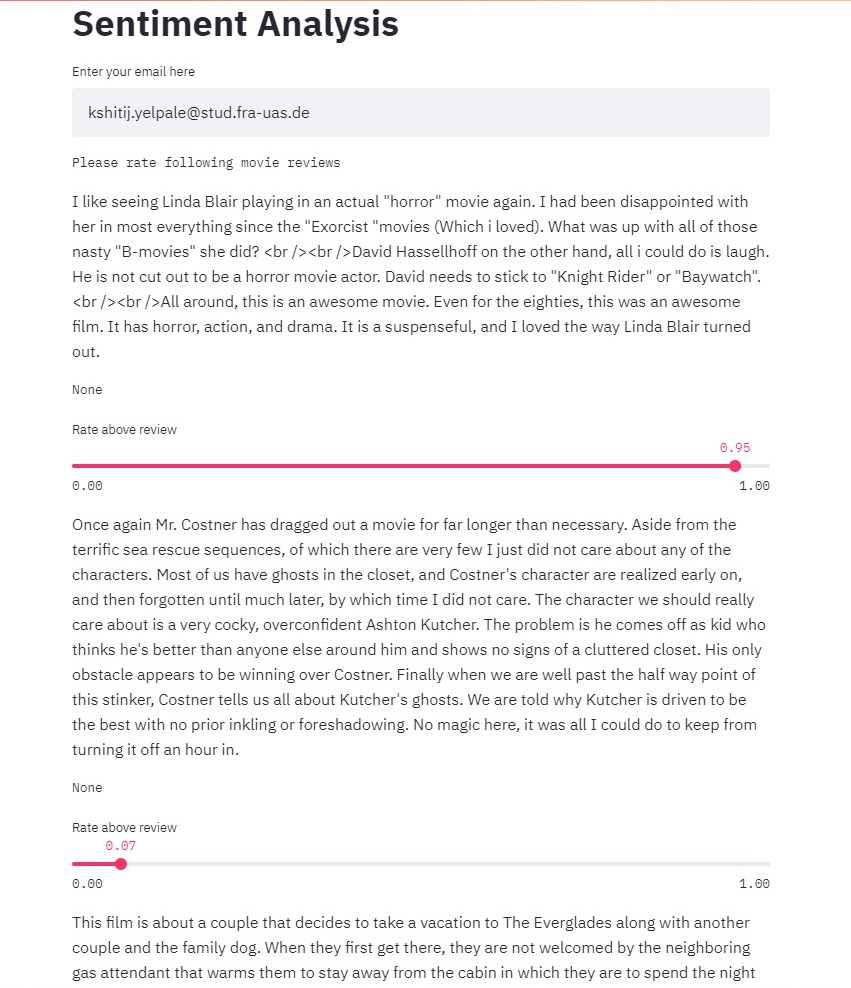
\includegraphics[width=8.5cm]{HMI_SC_1.jpg}
    \caption{}
    \label{fig:ss 1}
\end{figure}

\begin{figure}[h]
    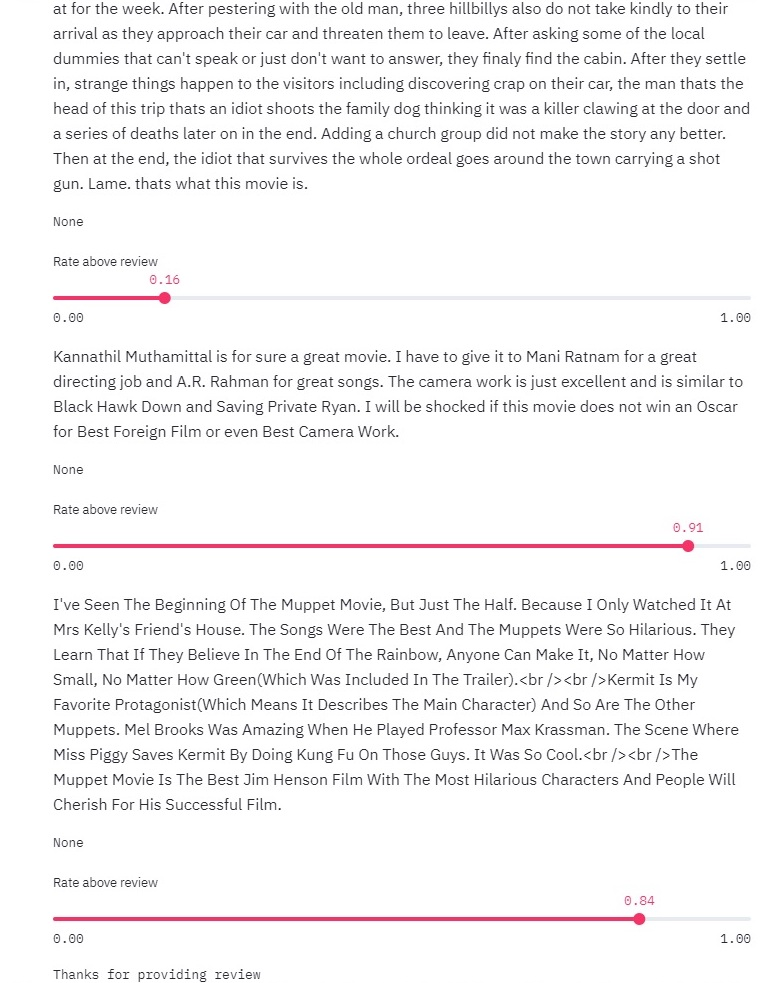
\includegraphics[width=8.5cm]{HMI_SC_2.jpg}
    \caption{}
    \label{fig:ss 2}
\end{figure}


\subsubsection{LSTM model:}
% The model is trained with 45000 IMDB movie reviews and validated and tested with 5000 documents. In data pre-processing, firstly we have removed stop words from the documents which do not express meaningful sentiments/which do not carry any meaning/weight-age in terms of Sentiment Analysis. Moreover, we have removed special characters and converted all words to lowercase. While creating the model, we have chosen the best optimization algorithm called "Adam". Since, Cross-Entropy is recommended for classification problems, we have used the same, i.e. "Binary Cross Entropy" in our case as we are aiming for 2 output classes. Also, we have saved the trained model and the corresponding weights so that we can use it later in any module by just loading the model without the need of training it every time for a long time.

Initilly, we developed 2 LSTM models which consisted of 3 layers, 
1. Embedding, 2. LSTM and 3. Dense. 
First with standard and well-processed Imdb dataset provided by keras library and other with custom Imdb dataset [17] having 50000 reviews. Both the dataset were well-splitted into training and validation data. We got 82.81\% and 81.29\% accuracy respectively. But we decided to go for a better model so that we might get better performance/results. Meanwhile, Keras also updated it's internal features and we had to face some challanges. 

Then with the same datasets, we built 2 Bidirectional LSTM models from which one fulfilled/served our purpose but the other one did not. So, finally, we came up with a Bi-LSTM model trained on Keras' inbuilt Imdb dataset and it gave 86.89\% accuracy. Before training, we dealt with data pre-processing techniques like Removing stopwords and special characters that does not carry any meaningful ingormation. Then, we converted the documents into lowercase and transformed the words into vectors of numbers in Imdb encoded format. This was one of our biggest research on converting the words into Keras encoded Imdb vector format. Next, we truncated/padded the documents with a fixed length of 200 words. We have also set the vocabulary size as 20000. The model contains 4 layers, 
1. Embedding, 2. BidirectionalLSTM X 2 and 3. Dense.

While creating the model, we have chosen the best optimization algorithm called "Adam". Since, Cross-Entropy is recommended for classification problems, we have used the same, i.e. "Binary Cross Entropy" in our case as we are aiming for 2 output classes. Also, we have saved the trained model and the corresponding weights so that we can use it later in any module by just loading the model (without the need of training again).


\subsubsection{Bayes model;}
We have created a generic text classifier that places the text of a movie review in one of two categories — negative or positive. We begin the process by performing text classification. Since texts are not understandable for machines, so we convert texts into numbers and this mechanism is called as Word Embedding. Here we used TF-IDF technique. This technique not only convert text to numbers but also signifies the importance of the term in the document. This model converts the text into numbers which is then used in the algorithm for analysis. 

Especially, this model is used to extract features from the text data and its significance. TF is term frequency which is calculated by no. of times the term appeared in the document divided by total no. of terms in the document. IDF is the common logarithm of total no. of documents to the no. of documents in which term exist. This is technique is important than other word embedding technique Bag of Words. The tf-idf value of a term or word is greater when more frequently it appears in document but less frequent in all documents. To achieve appropriate values of terms, one may use the techniques like stemming, lemmatization, converting to lower case or ignoring stop-words. We tokenized using TfidfVectorizer module of sci-kit-learn. analysis of Model is done in 4 steps.

\begin{figure}[h]
    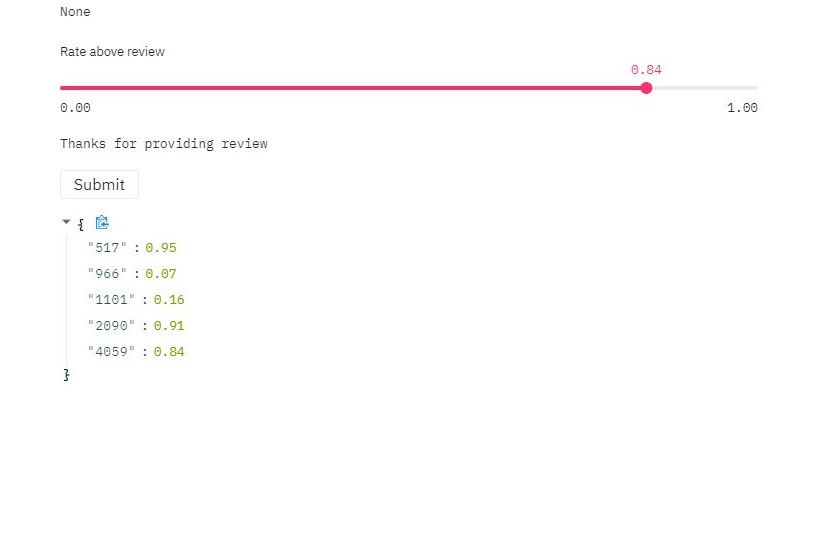
\includegraphics[width=8.5cm]{HMI_SC_3.jpeg}
    \caption{}
    \label{fig:ss 3}
\end{figure}

1. Model Definition 2. Compilation of the model 3. Fitting the model 4. Review the model

1. We used one of the Naive Bayes (NB) classifiers for defining the model. To be precise, we used MultinomialNaiveBayes classifier. MultinomialNaiveBayes allows to represent the features of the model as frequencies of their occurrences (i.e, how frequently a word occurs in our review). In other words, it tells us that the probability distributions that we are using is multinomial. 

2. To do this we used sklearn’s modules and classes. We have imported the precompiled classes. Sklearn gives information about all classes.
from sklearn. naive\_bayes import MultinomialNaiveBayes

3.In this step, we generated our model-fitting from our dataset in the MultinomialNaiveBayes.

Mnb=MultinomialNaiveBayes() 
Mnb.fit (X\_train, Y\_train)

4.In this step, we quantified the quality of our model. From sklearn library, we used metrics module to evaluate the predictions of the model.
From sklern import metrics
Predicted=Mnb.predict(X\_test)
Accuracy score=metrics. accuracy\_score (Predicted, Y\_test)


\subsection{Survey Procedure}
After giving informed consent, participants were asked to rate multiple long movie reviews through the user-interface of the web application. The users used the slider bars present under each review on the user interface to give the ratings on a scale of 0 to 1 (0 - negative, 1 - positive). After clicking on the submit button, the users were able to see the sentiments they assigned in a JSON format and the data was updated in the database. Difference between predicted values and value from participants were used to calculate the performance metric (deviation). This metric, in turn, was used for statistical testing.

\subsection{Participants}
We invited 10 computer science students from our institution and course High Integrity Systems (HIS) as participants for the study. Participants age ranged from 23 to 29 years (M = 25.7, SD = 1.64). All of them had a technical background in computer science and engineering. Responses were collected anonymously.


\subsection{Data Analysis}
A dataset of 4500 IMDB movie reviews (labeled: i.e. with actual sentiment values) were used for the purpose of analyses. This data was stored in a SQLite database. All the reviews were fed to both LSTM and Bayes models and their output recorded. 5 reviews were randomly selected and displayed to the user for rating. The user ratings were stored in database at user sentiments. Correlation was calculated for both LSTM and Bayes values with the actual values and results compared. The deviation of LSTM and Bayes values were calculated from actual sentiments. T-test was done to show that results were statistically significant.

\section{Results}
For hypothesis testing we calculated mean, standard deviation, correlation and performed 2-sampled T-test. We calculated the mean and standard deviation of the deviations of both LSTM and Bayes from the user sentiments. Mean(LSTM deviation) = 0.133, Mean(Bayes deviation) = 0.335. Standard deviation(LSTM) = 0.147, Standard deviation(Bayes) = 0.236.

We calculated the correlation of both the LSTM and Bayes values with the actual sentiment values from the labeled data. The Pearson correlation coefficient for LSTM = 0.882 and for Bayes = 0.001.
The Spearman correlation coefficient for LSTM = 0.886 and for Bayes = 0.002. Here it is clearly visible that LSTM has better correlation with the actual values than Bayes.

We performed 2-sampled T-test on LSTM deviations (deviations of LSTM values from user sentiment) and Bayes deviations (deviations of Bayes values from user sentiment). The p-value for 5\% significance = 1.432e-06. Since the p-value < significance level, we can reject the null hypothesis (H0: there is no significant difference between LSTM and Bayes deviations) and accept the alternate hypothesis (H1: there is significant difference between LSTM and Bayes deviations from user data).

All these statistical measures depict that LSTM based models are better for long textual sentiment classification as compared to Bayes based models.

\begin{figure}[h]
    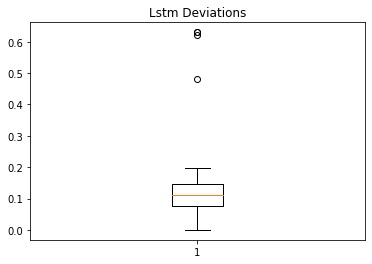
\includegraphics[width=8.5cm]{LSTM_boxPlot.jpeg}
    \caption{Box-Plot for LSTM deviations from user ratings}
    \label{fig:ss 1}
\end{figure}

\begin{figure}[h]
    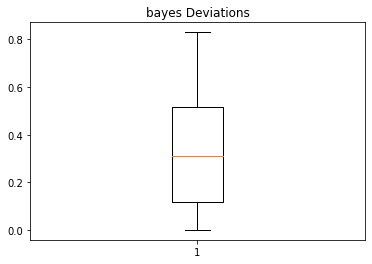
\includegraphics[width=8.5cm]{Bayes_boxPlot.jpeg}
    \caption{Box-Plot for Bayes deviations from user ratings}
    \label{fig:ss 1}
\end{figure}

\begin{figure}[h]
    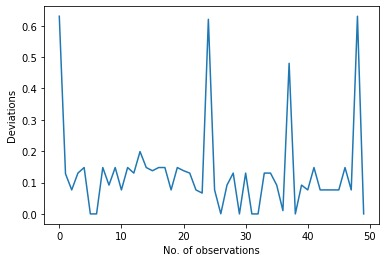
\includegraphics[width=8.5cm]{LSTM_Dev.jpeg}
    \caption{Plot for LSTM predicted values deviated from user ratings}
    \label{fig:ss 1}
\end{figure}

\begin{figure}[h]
    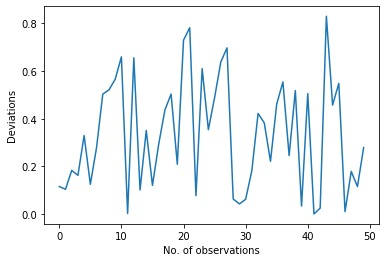
\includegraphics[width=8.5cm]{Bayes_Dev.jpeg}
    \caption{Plot for Bayes predicted values deviated from user ratings}
    \label{fig:ss 1}
\end{figure}

\section{Discussion}
After analysing the data collected in the experiment, we found that LSTM model gives good correlation values with the actual sentiments of the reviews whereas Bayes model correlation is not that strong. Conducting T-test on the deviations of both LSTM and bayes confirms that the difference is statistically significant. This proves that the null hypothesis (H0) can be rejected and alternate hypothesis (H1) can be accepted. This shows that LSTM is better choice as compared to bayes for sentiment analysis when it comes to long text reviews. This result is inline with the explaination that LSTMs are better in handling long sequences because of their recurrent nature.

\subsection{Future Work}
There is a lot of scope of extension to this research. The amount of data used for training the models and doing the evaluation can be increased. More participants can be involved for the evaluation part. There are various other models that can be compared against each other. Different types of data can be tested for various models. This research can further be used in actual applications like recommender systems. 



\begin{acks}
This research was possible under the guidance and direction of Prof. Dr. Valentin Schwind. This paper is the final report for the course Human Machine Interaction (HMI) taught in the Masters programme High Integrity Systems (HIS).
\end{acks}
%%
%% The next two lines define the bibliography style to be used, and
%% the bibliography file.


% \begin{table}[h]
%   \caption{table heading}
%   \label{tab:issue}
%   \begin{tabular}{c c c c c}
%     \toprule
%     Severity&P1&P2&P3&Total Unique Issues\\
%     \midrule
%     Critical&3&2&2&3\\
%     High&2&1&2&5\\
%     Low&6&8&6&8\\
%     Minor&5&3&4&12\\
%     SUBHAM&1&2&3&4\\
%   \bottomrule
%   &&&Total&28\\
% \end{tabular}
% \end{table}


\begin{thebibliography}{1}
\bibitem{IEEE}
K. Cho, B. V. Merrienboer, C. Bahdanau, F. Bougares, H. Schwenk,
and Y. Bengio. 2014. Learning phrase representations using RNN encoder–decoder for statistical machine translation. Technical Report. in
Proc. EMNLP, Doha, Qatar, 2014, pp. 1724–1734

\bibitem{IEEE}
Xianghua fu, Jingying yang, Jianqiang li, Min fang, and Huhui wang.
2018. Lexicon-Enhanced LSTM With Attention for General Sentiment
Analysis. Technical Report. Shenzhen University,Harbin Institute of
Technology, Shenzhen , China and Jacksonville University, Jacksonbville, FL 32211, USA.

\bibitem{IEEE}
Md. Rakibul Hasan, Maisha Maliha, and M. Arifuzzaman. 2019. Sentiment Analysis with NLP on Twitter Data. Technical Report. East
West University,Bangladesh University of Engineering and Technology, Dhaka.

\bibitem{IEEE}
S. Hochreiter and J. Schmidhuber. 1997. Long short-term memory.
Technical Report. Neural Comput., vol. 9, no. 8, pp. 1735–1780, 1997.

\bibitem{IEEE}
Ning Jin, Jiaxian Wu, Xiang Ma, Ke Yan, and Yuchang Mo. 2017. Multitask learning model based on Multi-scale CNN and LSTM for sentiment
classification. Technical Report. College of Information Engineering,
Jiliang University, Huaqiao University, Hangzhou, Quanzhou, China.

\bibitem{IEEE}
Y. Kim. 2014. SConvolutional neural networks for sentence classification.
Technical Report. https://arxiv.org/abs/1408.5882


\bibitem{IEEE}
Dan Li and Jiang Qian. 2016. Text Sentiment Analysis Based on Long
Short-Term Memory. Technical Report. Beijing University of Posts and
Telecommunications Beijing, China.

\bibitem{IEEE}
Yuan Lin, Jiaping Li, Liang Yang, Kan Xu, and Hongfei Lin2. 2017.
Sentiment Analysis with Comparison Enhanced Deep Neural Network.
Technical Report. Dalian University of Technology, Dalian, China.

\bibitem{IEEE}
A. L. Maas, R. E. Daly, P. T. Pham, D. Huang, A. Y. Ng, and C. Potts.
2011. Learning word vectors for sentiment analysis. Technical Report.
in Proc. ACL, Stroudsburg, PA, USA, 2011, pp. 142–150

\bibitem{IEEE}
T. Mikolov, K. Chen, G. Corrado, and J. Dean. 2013. Efficient estimation of word representations in vector space. Technical Report. https:
//arxiv.org/abs/1301.3781

\bibitem{IEEE}
Ms.R.Monika, Dr.S.Deivalakshmi, and Dr.B.Janet. 2019. Sentiment
Analysis of US Airlines Tweets using LSTM/RNN. Technical Report. Corrosion and Materials Protection Division CSIR-Central Electrochemical
Research Institute Karaikudi, National Institute of Technology Trichy,
India

\bibitem{IEEE}
O.Lev, Y.Goldberg, and I.Dagan. 2015. Improvingdistributionalsimilarity
with lessons learned from word embeddings. Technical Report. Trans.
Assoc. Comput. Linguistics,vol. 3, pp. 211–225, May 2015.

\bibitem{IEEE}
J. Pennington, R. Socher, and C. D. Manning. 2014. Glove: Global vectors
for word representation,. Technical Report. in Proc. EMNLP, vol. 14,
2014, pp. 1532–1543.

\bibitem{IEEE}
R. Socher, B. Huval, C. D. Manning, and A. Y. Ng. 2012. SSemantic
com- positionality through recursive matrix-vector spaces. Technical
Report. in Proc. EMNLP- CoNLL, Jeju Island, South Korea, 2012, pp.
1201–1211

\bibitem{IEEE}
R. Socher, J. Pennington, E. H. Huang, A. Y. Ng, and C. D. Manning.
2011. Semi-supervised recursive autoencoders for predicting sentiment
distri- butions. Technical Report. in Proc. EMNLP, Stroudsburg, PA,
USA, 2011, pp. 151–161.

\bibitem{IEEE}
 D. Y. Tang, F. Wei, N. Yang, M. Zhou, T. Liuand, and B. Qin. 2014.
Learning sentiment-specific word embedding for Twitter sentiment classification. Technical Report. in Proc. ACL, Baltimore, MD, USA, 2014,
pp. 1555–1565.

\bibitem{IEEE}
Andrew L. Maas, Raymond E. Daly, Peter T. Pham, Dan Huang, Andrew Y. Ng, and Christopher Potts. (2011). Learning Word Vectors for Sentiment Analysis. The 49th Annual Meeting of the Association for Computational Linguistics (ACL 2011).


\end{thebibliography}









%%
%% If your work has an appendix, this is the place to put it.
\appendix


\end{document}
\endinput
%%
%% End of file `sample-sigplan.tex'.